\documentclass[11pt,preprint, authoryear]{elsarticle}

\usepackage{lmodern}
%%%% My spacing
\usepackage{setspace}
\setstretch{1.2}
\DeclareMathSizes{12}{14}{10}{10}

% Wrap around which gives all figures included the [H] command, or places it "here". This can be tedious to code in Rmarkdown.
\usepackage{float}
\let\origfigure\figure
\let\endorigfigure\endfigure
\renewenvironment{figure}[1][2] {
    \expandafter\origfigure\expandafter[H]
} {
    \endorigfigure
}

\let\origtable\table
\let\endorigtable\endtable
\renewenvironment{table}[1][2] {
    \expandafter\origtable\expandafter[H]
} {
    \endorigtable
}


\usepackage{ifxetex,ifluatex}
\usepackage{fixltx2e} % provides \textsubscript
\ifnum 0\ifxetex 1\fi\ifluatex 1\fi=0 % if pdftex
  \usepackage[T1]{fontenc}
  \usepackage[utf8]{inputenc}
\else % if luatex or xelatex
  \ifxetex
    \usepackage{mathspec}
    \usepackage{xltxtra,xunicode}
  \else
    \usepackage{fontspec}
  \fi
  \defaultfontfeatures{Mapping=tex-text,Scale=MatchLowercase}
  \newcommand{\euro}{€}
\fi

\usepackage{amssymb, amsmath, amsthm, amsfonts}

\def\bibsection{\section*{References}} %%% Make "References" appear before bibliography


\usepackage[round]{natbib}

\usepackage{longtable}
\usepackage[margin=2.3cm,bottom=2cm,top=2.5cm, includefoot]{geometry}
\usepackage{fancyhdr}
\usepackage[bottom, hang, flushmargin]{footmisc}
\usepackage{graphicx}
\numberwithin{equation}{section}
\numberwithin{figure}{section}
\numberwithin{table}{section}
\setlength{\parindent}{0cm}
\setlength{\parskip}{1.3ex plus 0.5ex minus 0.3ex}
\usepackage{textcomp}
\renewcommand{\headrulewidth}{0.2pt}
\renewcommand{\footrulewidth}{0.3pt}

\usepackage{array}
\newcolumntype{x}[1]{>{\centering\arraybackslash\hspace{0pt}}p{#1}}

%%%%  Remove the "preprint submitted to" part. Don't worry about this either, it just looks better without it:
\makeatletter
\def\ps@pprintTitle{%
  \let\@oddhead\@empty
  \let\@evenhead\@empty
  \let\@oddfoot\@empty
  \let\@evenfoot\@oddfoot
}
\makeatother

 \def\tightlist{} % This allows for subbullets!

\usepackage{hyperref}
\hypersetup{breaklinks=true,
            bookmarks=true,
            colorlinks=true,
            citecolor=blue,
            urlcolor=blue,
            linkcolor=blue,
            pdfborder={0 0 0}}


% The following packages allow huxtable to work:
\usepackage{siunitx}
\usepackage{multirow}
\usepackage{hhline}
\usepackage{calc}
\usepackage{tabularx}
\usepackage{booktabs}
\usepackage{caption}


\newenvironment{columns}[1][]{}{}

\newenvironment{column}[1]{\begin{minipage}{#1}\ignorespaces}{%
\end{minipage}
\ifhmode\unskip\fi
\aftergroup\useignorespacesandallpars}

\def\useignorespacesandallpars#1\ignorespaces\fi{%
#1\fi\ignorespacesandallpars}

\makeatletter
\def\ignorespacesandallpars{%
  \@ifnextchar\par
    {\expandafter\ignorespacesandallpars\@gobble}%
    {}%
}
\makeatother

\newlength{\cslhangindent}
\setlength{\cslhangindent}{1.5em}
\newenvironment{CSLReferences}%
  {\setlength{\parindent}{0pt}%
  \everypar{\setlength{\hangindent}{\cslhangindent}}\ignorespaces}%
  {\par}


\urlstyle{same}  % don't use monospace font for urls
\setlength{\parindent}{0pt}
\setlength{\parskip}{6pt plus 2pt minus 1pt}
\setlength{\emergencystretch}{3em}  % prevent overfull lines
\setcounter{secnumdepth}{5}

%%% Use protect on footnotes to avoid problems with footnotes in titles
\let\rmarkdownfootnote\footnote%
\def\footnote{\protect\rmarkdownfootnote}
\IfFileExists{upquote.sty}{\usepackage{upquote}}{}

%%% Include extra packages specified by user

%%% Hard setting column skips for reports - this ensures greater consistency and control over the length settings in the document.
%% page layout
%% paragraphs
\setlength{\baselineskip}{12pt plus 0pt minus 0pt}
\setlength{\parskip}{12pt plus 0pt minus 0pt}
\setlength{\parindent}{0pt plus 0pt minus 0pt}
%% floats
\setlength{\floatsep}{12pt plus 0 pt minus 0pt}
\setlength{\textfloatsep}{20pt plus 0pt minus 0pt}
\setlength{\intextsep}{14pt plus 0pt minus 0pt}
\setlength{\dbltextfloatsep}{20pt plus 0pt minus 0pt}
\setlength{\dblfloatsep}{14pt plus 0pt minus 0pt}
%% maths
\setlength{\abovedisplayskip}{12pt plus 0pt minus 0pt}
\setlength{\belowdisplayskip}{12pt plus 0pt minus 0pt}
%% lists
\setlength{\topsep}{10pt plus 0pt minus 0pt}
\setlength{\partopsep}{3pt plus 0pt minus 0pt}
\setlength{\itemsep}{5pt plus 0pt minus 0pt}
\setlength{\labelsep}{8mm plus 0mm minus 0mm}
\setlength{\parsep}{\the\parskip}
\setlength{\listparindent}{\the\parindent}
%% verbatim
\setlength{\fboxsep}{5pt plus 0pt minus 0pt}



\begin{document}



\begin{frontmatter}  %

\title{Revisiting What Caused The Early Millenium Slowdown}

% Set to FALSE if wanting to remove title (for submission)




\author[Add1]{Jessica Van der Berg}
\ead{20190565@sun.ac.za}





\address[Add1]{20190565}



\vspace{1cm}

\begin{keyword}
\footnotesize{
Vectorautoregressive process\sep Millenium Slowdown\sep Time Series
Analysis \\ \vspace{0.3cm}
\textit{JEL classification} 
}
\end{keyword}
\vspace{0.5cm}
\end{frontmatter}



%________________________
% Header and Footers
%%%%%%%%%%%%%%%%%%%%%%%%%%%%%%%%%
\pagestyle{fancy}
\chead{}
\rhead{A replication of Gert Peersman (2005) paper}
\lfoot{}
\rfoot{\footnotesize Page \thepage}
\lhead{}
%\rfoot{\footnotesize Page \thepage } % "e.g. Page 2"
\cfoot{}

%\setlength\headheight{30pt}
%%%%%%%%%%%%%%%%%%%%%%%%%%%%%%%%%
%________________________

\headsep 35pt % So that header does not go over title




\hypertarget{introduction}{%
\section{Introduction}\label{introduction}}

In this research assignment, I replicate a research assignment by Gert
Peersman (2005), a German economist, titled ``What caused the early
millennium slowdown? Evidence based on vector autoregressions''. In this
paper, Peersman (2005) uses a simple four-variable VAR (vector
autogressive model) and an identification based scheme based on sign
restrictions to examine the effects of a supply, demand, monetary policy
and oil price shocks. Peersman (2005) uses data from the United States
(US) and Euro area. However, this assignment will only focus on
analyzing shocks for the US. Peersman (2005) concludes that the
millennial slowdown is not the result of one particular shock, but a
combination of them. The goal of this assignment is to replicate the
results of Peersman (2005) as well as preform additional robustness test
to ensure the validity of Peermans (2005) results.

This paper is structured as follows: The second section will give an
overview of the paper with respects to the economics, methodology and
data that Peersman (2005) used. The third section will replicate the
impulse response functions for the US, commenting on any difference
found. The four section will perform several diagnostics and robustness
checks and the forth section will reach the conclusion that Peersman
(2005) chose an appropriate model for his analysis.

\hypertarget{overview-of-the-paper}{%
\section{Overview of the paper}\label{overview-of-the-paper}}

This section gives a brief overview of the economics of the paper that I
am replicating as well as a critical evaluation of the statistical
approach that Peersman (2005) choose to analyze possible causes for the
economic slowdown of the US.

\hypertarget{theory-of-paper}{%
\subsection{Theory of Paper}\label{theory-of-paper}}

The 1990s was the start of an economic boom for the United States (US)
as they experienced the unusual combination of rapid output growth and
extremely low and stable inflation. From 1994 to 2002 the US real GDP
grew by an average annual rate of almost 4 percent while annual
inflation was less than 2 percent. However, by the end of 2001, the US
began to experience negative growth (Peersman, 2005). Since 2001, the US
economy has not experienced close to the same economic growth as before.
It is therefore important to understand what caused the slowdown.

The economic expansion that the US experienced made headlines as it was
the longest expansion in economic history. Many explanations have been
offered as to why the US experienced such rapid growth, but overall, it
is attributed to numerous factors. Productivity growth increased
tremendously which created a favorable investment environment. The
private investment opportunities contributed to the advancements in
technologies and inspired innovation (Weller, 2002). Furthermore, the
Federal Open Market Committee (FOMC) created an environment for the
Federal Reserve to keep inflation rates low and stable (Taylor, 1998).

Another possible reason is that the US economy mostly experienced
positive shocks during the late 1990s. The Fed has the responsibility to
responds to shocks to the economy to ensure that output, employment, and
inflation remain stable. The Fed can easily respond to a demand shock as
it pushed output, employment, and inflation in the same direction.
Therefore, the Fed will lower interest rate which will increase money
supply to combat the effects of a demand shock. However, a supply shock,
such as an increase in oil prices, are more complicated to respond to.
With the threat of a recession, the Fed will need to decide whether to
prioritize inflation stability or employment stability. The fact that
large supply shocks were uncommon during the 1990s was also a factor
that greatly influenced the economic boom that the US experienced.

After 10 years of economic growth, the US economy entered into a
recession. The 2001/2002 recession was relatively short lived. Kliesen
(2003) argues that the recession was caused by shocks to investment by
businesses and households and by a decline in real net exports. However,
Kleisen (2003) does recognize that it can be extremely difficult to
challenging to discover the root cause of a recession. Understanding
fluctuation that effect the growth of an economy has been researched by
many economists but it is still relatively poorly understood. Therefore,
Peersman (2005) adds value to existing research by examining four shocks
(oil, demand, supply, and monetary policy) to analyze the origin of the
slowdown.

Peersman (2005) concludes that the slowdown of economic growth was
caused by a combination of several shocks. This conclusion is
non-surprising and therefore Peersman (2005) main contribution is the
impressive mathematical and statistical analysis that he performed. This
analysis is discussed in the next section.

\hypertarget{data-and-methodology}{%
\subsection{Data and Methodology}\label{data-and-methodology}}

This paper used quarterly data from 1980 to 2002 on the US consumer
expenditure index (CPUS), real GDP (YUS), short term nominal interest
rate (SUS) as well as data on the oil price (OIL). Changes in CPUS
record the rate of consumer inflation while changes in YUS record output
growth. The data is then manipulated to display the first difference of
the log of OIL, YUS and CPUS and these variables are assumed to be I(1)
variables. A I(1) variables means that orginally the data is
non-stationary, but now that it has been differenced and demeaned, the
data is stationary. The SUS variable is taken as an I(0) variable
(Ouliaris, Pagan \& Restrepo, 2018). The data is presented in figure 2.1
below.

\begin{figure}[H]

{\centering 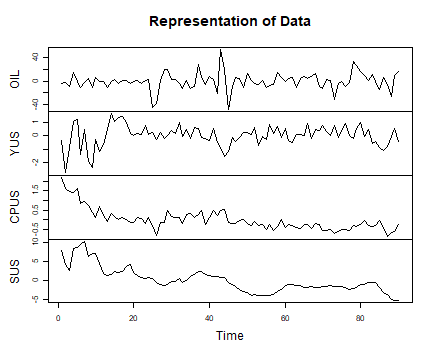
\includegraphics{replication_files/figure-latex/Figure1-1} 

}

\caption{Data\label{Figure1}}\label{fig:Figure1}
\end{figure}

Peersman (2005) estimates a four-variable constant-coefficient vector
autoregression (VAR) model, with three lags and identifies four shocks.
The four shocks that are analyzed in this paper are; two supply shocks,
one demand shock and one monetary policy shock. The two supply shocks
represents a shock to the oil price and a shock to output growth. The
demand shock is associated with a shock to consumer inflation, while the
monetary policy shock is associated with a shock to the short term
nominal interest rate. Taking the four variables and shocks into
account, the equation can be presented as follows:

\[\begin{bmatrix} \Delta oil_t \\ \Delta y_t \\ \Delta p_t \\ s_t \end{bmatrix} = \Biggl[ I - \sum_{i=1}^{n} A_i \Biggl]^{-1} \begin{bmatrix} b_{11}& b_{12}& b_{13} & b_{14} \\
b_{21}& b_{22}& b_{23} & b_{24} \\
b_{31}& b_{32}& b_{33} & b_{34} \\
b_{41}& b_{42}& b_{43} & b_{44} \end{bmatrix} \begin{bmatrix} \epsilon_t^{oil} \\ \epsilon_t^{s} \\ \epsilon_t^{d} \\ \epsilon_t^{m} \end{bmatrix}\]

Where \(\Delta oil_t\), \(\Delta y_t\) and \(\Delta p_t\) represent the
first difference of the price of oil, output growth and the consumer
prices respectively. \(s_t\) represents the short term nominal interest
rate. The oil price, demand, supply and monetary shock in represented by
\(\epsilon_t^{oil}\), \(\epsilon_t^{d}\), \(\epsilon_t^{s}\) and
\(\epsilon_t^{m}\) respectively.

Peersman (2005) assumes that the variables follow a covariance
stationary process. He uses the Dickey fuller test to reject the null
hypothesis of the existence of a unit root at a 10 percent level for
OIL, YUS and CPUS, however, the null hypothesis for interest rates
cannot be rejected. Peersman (2005) makes the assumption that interest
rates are stationary since the nominal rate cannot have a unit root if
both the real rate and inflation are stationary. This assumption will be
intensely analyzed in section 4 during which I will preform numerous
robustness checks.

The paper makes use of a traditional identification strategy using a
combination of short-run and long-run restrictions. Peersman (2005)
assumes that there is a contemporaneous impact of an oil shock on all
variables in the structural VAR (SVAR), but no immediate impact of other
shocks on oil prices. This assumption is consistent with previous
literature. Further Peersman (2005) adds the restrictions that a
monetary policy shock has no contemporaneous effect on output, since
monetary policy shocks have a temporary effect on output. To model these
contemporaneous effects \(b_{12} = b_{13} = b_{14} = b_{24} = 0\).
However, to accurately model the contemporaneous effects, the SVAR needs
\([k^2-k]/2\) restrictions, where k represents the number of variables.
This implies that a further two restrictions are needed in order to
model the VAR successfully, which will be long run restrictions. The
contemporaneous matrix that include only short run restrictions is
presented below;

\[\ \begin{bmatrix} b_{11}& 0 & 0 & 0 \\
b_{21}& b_{22}& b_{23} & 0 \\
b_{31}& b_{32}& b_{33} & b_{34} \\
b_{41}& b_{42}& b_{43} & b_{44} \end{bmatrix} \]

Peersman (2005) follows Blanchard and Quah (1989), Gali (1992) and
Gerlach and Smeth (1995) to add long-run restrictions to the model. He
assumes that demand shock has a permanent zero long-run effect of output
growth YUS. Furthermore, Peersman (2005) assumes that monetary shocks
has a zero long-run impact on output growth but a non-zero effect of OIL
and CPUS. Therefore, your long-run restriction matrix will be
represented as follow;

\[\ \begin{bmatrix} *& *& *& * \\
*& *& 0 & 0 \\
*& *& *& * \\
*& *& * & * \end{bmatrix} \]

where the zero's represent the restrictions. In the next section, I
replicate and evaluate the impulse response functions that are
correlated with the VAR specified by Peersman (2005).

\hypertarget{replication}{%
\section{Replication}\label{replication}}

In this section, I use Peersman (2005) data on the US to evaluate the
SVAR by plotting impulse response function, 40 periods ahead, with an
84th and 16th percent confidence band. In Peersman (2005) paper, he
applies four short run restrictions to his SVAR and two long-run
restrictions, adding up to the necessary 6 restrictions that is needed
for the evaluation. In this section, I examine each variables response
to the different shocks and compare them to Peersman (2005) results
\footnote{Peersman (2005) original results are displayed in appendix A}.

Under the restrictions specified by Peersman (2005), an oil price shock
is interpreted as an shock to oil price (OIL), a demand shock is
interpreted as a shock to the consumer expenditure index (CPUS), a
supply shock is interpreted as a shock to output growth (YUS) and a
monetary policy shock is interpreted as a shock to the short term
nominal interest rate (SUS).

\hypertarget{oils-response}{%
\subsection{Oil's response}\label{oils-response}}

Oil is one of the most important commodities in the world. A lower oil
price benefits consumer as it provides cheaper traveling cost and a
lower price of gasoline. The oil price also impacts the price of many
manufactured goods, therefore it affects every consumer. Thus, it is
important to understand how the oil price will respond to different
types of shocks. Figure 3.1 shows that there is a permanent effect on
the price of oil for all shocks. The oil price increases after a
positive demand shock and decrease for a restrictive monetary policy
shock. A positive oil shock increases the price of oil. These impulse
response functions replicate Peersman (2005) results.

There is also a permanent effect on the price of oil for a supply shock,
which contradicts Peersman (2005) results as he found only a temporary
increase in the price of oil after a supply shock. Theoretically, demand
and supply shocks have different impacts on the price of oil, where
demand shocks are usually more persistent with a larger impact than
supply shocks. However, in Figure 3.1, it is observed that they have
similar impacts. Therefore, based on my results and Peersman (2005)
results, I argue that the effects of a supply shock on oil price is
ambiguous.

\begin{figure}[H]

{\centering 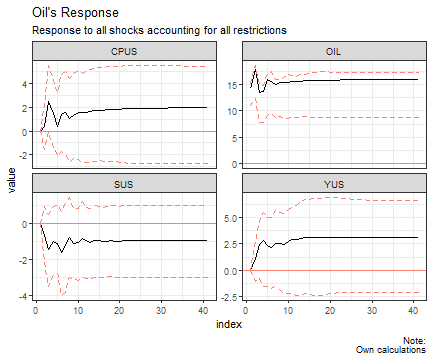
\includegraphics{replication_files/figure-latex/Figure2-1} 

}

\caption{Response of Oil Price\label{Figure2}}\label{fig:Figure2}
\end{figure}

\hypertarget{output-growth-response}{%
\subsection{Output Growth Response}\label{output-growth-response}}

To implemented the long-run restrictions specified by Peersman (2005) on
output growth, I implement an identification scheme proposed by
Blanchard-Quah (1989). In Blanchard-Quah original model, the assumption
is made that demand shock has no effect on the long run levels of
output. Peersman (2005) makes the same assumption is his papers and also
assumes that monetary policy shocks have no impact on output growth in
the long run. As can be seen in Figure 3.2, my results for the response
of outgrowth for different shocks are an exact replication of Peersman
(2005) results.

Figure 3.2 shows that output growth responds negatively to an oil shock,
and positively to a demand and monetary policy shock. Additionally, a
demand and monetary policy shock only have a temporary effect on output
growth where the effect of a demand shock is longer lasting. Therefore,
a monetary policy shock has a rather insignificant effect on output
growth where as a demand shock boost economic growth.

\begin{figure}[H]

{\centering 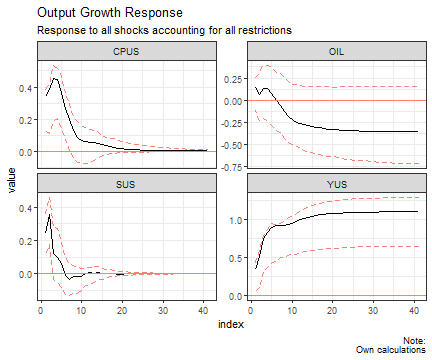
\includegraphics{replication_files/figure-latex/Figure3-1} 

}

\caption{Response of Output growth\label{Figure3}}\label{fig:Figure3}
\end{figure}

\hypertarget{consumer-expenditure-index-response}{%
\subsection{Consumer Expenditure Index
Response}\label{consumer-expenditure-index-response}}

Figure 3.3 shows the response of consumer inflation to all four shocks.
These results are identical to Peersman (2005) results except for the
effect of a monetary policy shock on inflation. An oil shock and a
demand shock has a strong, positive, long run effect on consumer prices.
This makes theoretical sense, a demand shock insinuates that consumers
want to consumer more, hence they are willing to pay more and therefore
inflation increases. Furthermore, Gao, Kim, and Saba (2014) found a
positive effect of an oil price shock on total CPI which in mainly
attributed to the positive effect on energy intensive CPI. Therefore,
Goa, Kim and Saba (2014) supports Peersman (2005) results.

A supply shock has a strong, negative long-run effect on consumer
inflation. One example of this is when an positive supply shock occurs
due to an increase in money supply. This benefits consumers and
institutions in the short run but as a negative long run effect since
money purchasing power decreases. On the other hand, a monetary policy
shock seems to have no long-run impact on inflation. This result is
concerning as it contradicts Peersman (2005) results of a permanent
negative effect on inflation.

\begin{figure}[H]

{\centering 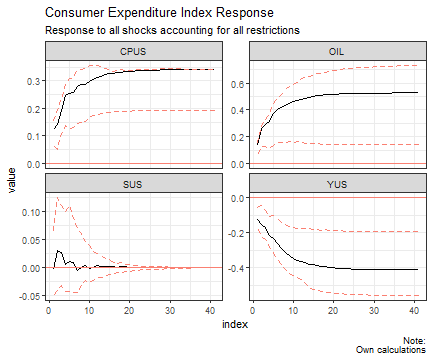
\includegraphics{replication_files/figure-latex/Figure4-1} 

}

\caption{Consumer Expenditure Index\label{Figure4}}\label{fig:Figure4}
\end{figure}

\hypertarget{short-term-nominal-interest-rate-response}{%
\subsection{Short Term Nominal Interest Rate
Response}\label{short-term-nominal-interest-rate-response}}

Figure 3.4 is an exact replication of Peersman (2005) result. All shocks
have a temporary, positive effect on interest rates. The pass through of
an oil and demand shock is longer lived than that of a monetary and
supply shock. An oil shock increases interest rates temporarily to
counterbalance the inflationary pressure.

The results are consistent with past literature. Gerlach and Smets
(1995) concluded that a monetary policy shock has a positive effect on
interest rates. However they found that the interest rates return to
starting state at a much faster then what is shown in figure 3.4.
Further, they found that interest rates increase after an demand shock
for the US and and concluded that an positive supply shocks increase the
return to capital and therefore real interest rates.

\begin{figure}[H]

{\centering 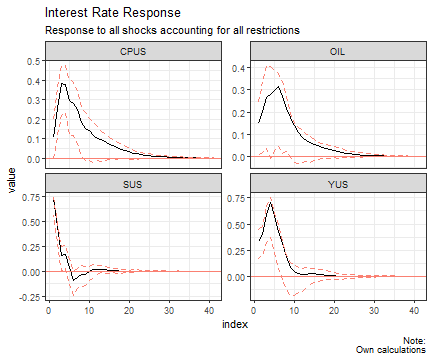
\includegraphics{replication_files/figure-latex/Figure5-1} 

}

\caption{Interest Rate Response\label{Figure5}}\label{fig:Figure5}
\end{figure}

\hypertarget{robustness-checks}{%
\section{Robustness checks}\label{robustness-checks}}

After replicating Peersman (2005) paper, I will now apply numerous
diagnostic and robustness test to determine whether a four-variable
SVAR(3) is an accurate representation of the data generating process. I
first analyze the optimal lag length for the model and then critically
test for stationarity. I will first test for the optimal lag length and
then preform several test to determine whether the variables are
stationary. After, I preform three diagnostic test on residuals which is
followed by a granger causality test. Lastly, I evaluate and plot the
forecast error variance decomposition.

\hypertarget{optimal-lag-length}{%
\subsection{Optimal lag length}\label{optimal-lag-length}}

Estimating a lag length for a VAR time series model is a critical
econometric exercise as one runs the risk of over or under estimation
(Liew, 2004). The model specified in the paper uses a lag length of 3.
There are four different criteria that one can analyze to decided on an
optimal lag length: the Akaike Information Criterion (AIC), the Schwarz
Criterion (SC), the Hannan Quinn (HQ) and the Final Prediction Error
(FPE).

As can be seen in the table below, Peersman (2005) chooses the FPE lag
criteria for an optimal lag length. The table also shows that there is a
large discrepancy between the VAR(10) selected by the AIC and the VAR(1)
and VAR(3) selected by the other criteria. This result is not unusual as
AIC usually chooses a larger number of lags. Therefore, it is preferred
to not use the AIC criteria when choosing a number a lags.

\begin{center}
\begin{tabular}{ |c|c|c|c| } 
 \hline
 AIC(n) & HQ(n) & SC(n) & FPE(n) \\ 
 \hline
 10 & 1 & 1 & 3\\ 
 \hline
\end{tabular}
\end{center}

Liew (2004) conducted a study where he critically analyzed which lag
length criteria should be used to determine the VAR lag length. He
concluded that AIC and FPE produce the least probability of under
estimation when compared to the other selection criteria. Since I have
already argued that AIC is not the best lag length criteria for this VAR
model, I agree with Peersman (2020) choice of using FPE to decide on a
lag length of three.

\hypertarget{test-for-stationary}{%
\subsection{\texorpdfstring{Test for Stationary
\label{stationary}}{Test for Stationary }}\label{test-for-stationary}}

Stationarity is a dominant principle in time series analysis. Stationary
implies that the statistical properties of a time series variable do not
change over time. It is important to know whether your variables are
stationary as many of the econometric test that you preform require
variables to be stationary. To analyze whether the data is stationary, I
plot the autocorrelation function (ACF) for each variable. On the x-axis
you will have the number of lags and on the y-axis you will have your
autocorrelation value. If the variable is stationary, the ACF will
degrade to zero quickly, whereas if they are non-stationary they will
slowly diminish as the number of lags increase. As seen in figure 4.1
below, the ACF plot implies that OIL and YUS are stationary variables
where CPUS and SUS are non-stationary variables.

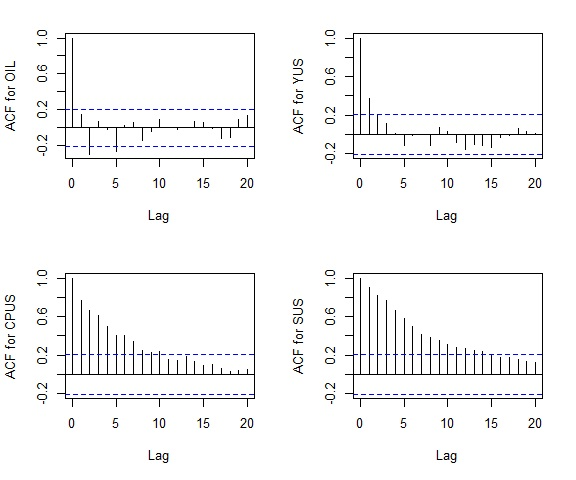
\includegraphics{ACF.jpg} To further investigate the stationarity of the
dataset, I preform the Augmented Dickey Fuller (ADF) test, with no trend
since we detrended our variables. The ADF test is a unit root test for
stationarity. I want to test for a unit root since a unit root can bring
about an unpredictable result in time series analysis. The ADF test null
hypothesis is that there is a unit root present, where the alternative
hypothesis is that the time series is stationary. The results of the ADF
test are given in the table below:

\begin{center}
\begin{tabular}{ |c|c|c| } 
 \hline
 variable & ADF statistic & P-value \\ 
 \hline
 OIL & -5.02 & 0.01\\ 
 YUS & -4.50 & 0.01 \\
 CPUS & -3.64 & 0.01 \\
 SUS & -1.09 & 0.2859 \\
 \hline
\end{tabular}
\end{center}

From this table, we can reject the null hypothesis of a unit root being
present for OIL, YUS and CPUS implying that the variables are
stationary, but we fail to reject the null hypothesis for SUS. The ADF
test results need to be interpreted with caution since it has a high
probability of a type I error rate. A type I error is the false
rejection of the null hypothesis. Therefore, I also make use of another
unit root test, the Phillips-Perron (PP) test.

The PP test corrects for any serial correlation and heteroskedasticity
by building onto the ADF results. Although the ADF test are more widely
used, the PP tests are more robust to general forms of
heteroskedasticity in the error term. Therefore, it is an appropriate
statistic to analyze to determine stationarity. The null hypothesis is
the same as the ADF test, that the time series has a unit root, where
the alternative hypothesis would be that the time series is stationary.
The results for the PP test is displayed in the table below.

\begin{center}
\begin{tabular}{ |c|c|c| } 
 \hline
 variable & PP statistic & P-value \\ 
 \hline
 OIL & -66.5 & 0.01\\ 
 YUS & -56.3 & 0.01 \\
 CPUS & -17 & 0.01 \\
 SUS & -7.25 & 0.0632 \\
 \hline
\end{tabular}
\end{center}

Analyzing the results for the PP test, we reach the exact same
conclusion as with the ADF test. Therefore, after plotting the
autocorrelation function and analyzing two unit root test, we reach the
same conclusion that Peersman (2005) reached in his paper. For OIL, YUS
and CPUS we reject the null hypothesis of a unit root and concluded that
the time series variables are stationary, even though the ACF shows
contradicting results for CPUS.

In all three test preformed, the same conclusion is reached regarding
the status of SUS, which is that it is non-stationary. However, Peersman
(2005) comes to the same conclusion. Gerlach and Smets (1995) agrue that
the nominal rate cannot have a unit root when both the real rate and
inflation are stationary. Therefore, the non-stationary result is not of
concern.

\hypertarget{diagnostic-test-on-residuals}{%
\subsection{Diagnostic Test on
Residuals}\label{diagnostic-test-on-residuals}}

To evaluate the model fit, I preform three diagnostic test on the
residuals of the model. The first test I preform is a test for white
noise residuals using the Portmanteau-test, which test for serial
correlation between errors. The null hypothesis is that the errors are
white noise, meaning that they are serially uncorrelated and that each
error has an identical, independent, mean-zero distribution. The
alternative hypothesis is therefore that the errors are serially
correlated. I run the Portmanteau-test for 12 lags and obtain a p-value
equal to 0.573. Therefore, I fail to reject the null hypothesis. This
means that the variables are a white noise process which supports
Peersman (2005) use of a VAR(3) model.

For the second diagnostic test I preform a multivariate
ARCH\footnote{ARCH stands for Autoregressive Conditional Heteroscedasiticity}-Lagrange-Multiplier
test for heteroscedasticity. The alternative hypothesis is that
autocorrelation is present in the squared residuals, therefore the null
hypothesis is the absence of autoregressive conditional
heteroscedasticity. The p-value is greater then 5 percent, implying that
there is no heteroscedasticity present. This conclusion supports
Peersman (2005) choice of a VAR(3) model.

The final diagnostic test on residuals that I preform, is a test for
structural breaks where I apply a cumulative sum (CUSUM) test. If a
structural break is present, it could imply that a four variable VAR(3)
is not the optimal model to use. In figure xx, I plot each variables
empirical fluctuation process to see whether a structural break is
present. A structural brake will occur if the fluctuations exceed the 95
percent confidence band. Studying figure xx, there does not seem to be a
break in the respective confidence intervals. Therefore, there is no
enough evidence to disapprove of the use of a four variable VAR(3)
model.

\begin{figure}[H]

{\centering 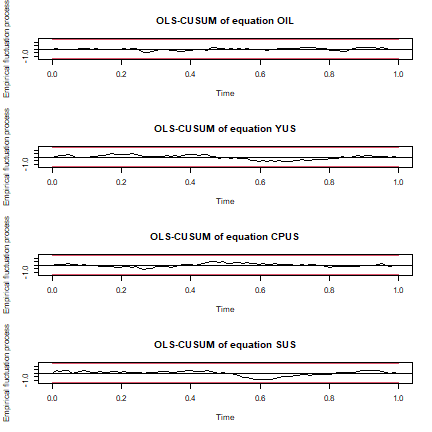
\includegraphics{replication_files/figure-latex/Figure8-1} 

}

\caption{Test for Structural Break\label{Figure8}}\label{fig:Figure8}
\end{figure}

\hypertarget{granger-causality}{%
\subsection{Granger Causality}\label{granger-causality}}

We would now like to know whether changes in one variable will have a
effect on changes in other variables in the dataset. The granger
causality test is a test done to determine whether on time series
variable is useful in forecasting another. We say that one time series
variables (x) granger-causes another time series variable (y) if it
depends on its own past values as well as the past values of x. For
predicting y, we then need to look at the past values of y and the past
values of x. The null hypothesis for the Granger Causaily test is that
the variable specified does not granger-cause any of the other variables
in the dataset. The results are shown in the table below.

\begin{center}
\begin{tabular}{ |c|c|c| } 
 \hline
 cause variable & F-stat & P-value \\ 
 \hline
 OIL & 2.8941 & 0.002711\\ 
 YUS & 3.5067 & 0.0003864 \\
 CPUS & 6.9537 & 4.293e-09\\
 SUS & 4.4792 & 1.5995-o5 \\
 \hline
\end{tabular}
\end{center}

For all cause variables, we reject the null hypothesis that the
cause-variable does not granger-cause on any of the other time series
variables.Therefore, we can derive the following results:

\begin{enumerate}
\item The hypothesis that the oil price does not influence the real GDP index, the consumer expenditure index and the short term nominal interest rate is rejected. This implies that the oil price does influences the US economy. 
\item The hypothesis that the real GDP index does not influence oil price, the consumer expenditure index and the short term nominal interest rate is rejected. This implies that real GDP has an effect on the US economy as well as the oil price, which greatly affects countries that are net importers of oil. 
\item The hypothesis that the consumer expenditure index does not influence the real GDP index, the oil price and the short term nominal interest rate is rejected. This implies that the US citizens spending patterns and behaviors affect the US economy as well as the oil price. 
\item The hypothesis that the short term nominal interest rate does not influence the real GDP index, the consumer expenditure index and the oil price is rejected. This implies that monetary policy greatly affects the US economy and has an affect on the oil price.
\end{enumerate}

\hypertarget{forecast-error-variance-decomposition}{%
\subsection{Forecast Error Variance
Decomposition}\label{forecast-error-variance-decomposition}}

Now that we have determined that all the variables granger-cause each
other, we can decompose the variance of the forecast error to determine
the impact of the contribution from the shocks specified in the
paper.This is done through using the forecast error variance
decomposition (FEVD) method.The FEVD plot below displays how important
shocks are for explaining variation in the variables. It also gives us a
time analysis of the important of certain shocks. For example, for
output growth, a monetary shock is not responsible for variation in the
short term but it does cause longer term fluctuations.

The results displayed in figure 4.2 suggest that oil is largely
determined by oil shocks Output growth is mostly determined by supply
shock but monetary policy shock also has a significant influence on
output growth. Inflation is mostly determined by an oil price shock and
a demand shock. Interest rates are largely determined by all four shock
specified in the model, where a supply shock has the most significant
effect on it and a monetary policy shock has a diminishing effect.

\begin{figure}[H]

{\centering 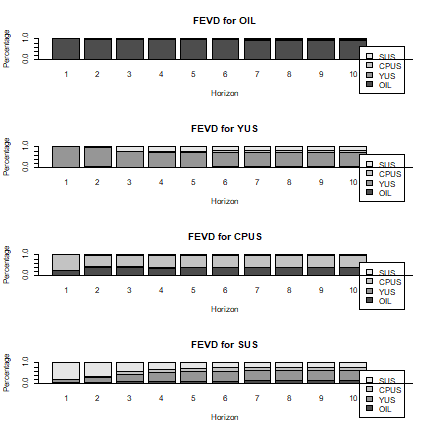
\includegraphics{replication_files/figure-latex/r Figure9-1} 

}

\caption{Forcast error variance decomposition\label{Figure9}}\label{fig:r Figure9}
\end{figure}

\hypertarget{conclusion}{%
\section{Conclusion}\label{conclusion}}

This paper sets out to replicates Peersman (2005) results by analyzing
the same data set from the US and estimating a four-variable VAR(3)
model considering short run and long run restrictions simultaneously. To
analyze the model, the impulse response function are graphed taking into
account four shocks; an oil price, demand, supply and monetary policy
shock. These shocks area associated with the four variables; oil price,
consumer inflation, output growth and short term nominal interest rate,
respectively. I successfully managed to replicate Peersman's results
except for two impulse response functions. The first being the a supply
shock to oil and the second being a supply shock to consumer inflation.
Supply shocks can be challenging to model and interpret since such a
shock tend to change the output-inflation combination in the economy.

After I replicated Peersman results, I preform numerous robustness test
to determine whether a four-variable VAR(3) is a sufficient and accurate
model to estimate. I first analyze the optimal lag length by studying
four different criteria and conclude that 3 lags is optimal. Secondly, I
test whether the variables in the data set are stationary by studying
the autocorrelation function, the augmented dickey fuller test and the
Philips-Perron test. I concluded that 3 YUS, CPUS and OIL is
stationarity, however SUS is non stationary. It can be argued
theoretically that SUS is stationary, therefore the results are not
concerning. I then preform three diagnostic tests on the residuals on
the VAR(3) and find no evidence that disproves of the model. Fourthly, I
prefrom the granger causality test to determine whether variables in the
model granger-cause eachother. The results were no surprising as
macroeconomic variables often affect eachother. Lastly, I plot the
forecast error variance decomposition to accurately analyze which
variables are affected by which results.

I therefore find no evidence to disprove the four-variable VAR(3) that
Peersman used in his paper. The results from the robustness checks prove
that the model is accurate and robust. Peersman correctly specified his
model taking into account the non-stationarity of one of the variables.

word count {[}4171{]}

\newpage

\hypertarget{references}{%
\section*{References}\label{references}}
\addcontentsline{toc}{section}{References}

Blanchard, O.J., 1989. A traditional interpretation of macroeconomic
fluctuations. The American Economic Review, pp.1146-1164.

Gao, L., Kim, H. and Saba, R., 2014. How do oil price shocks affect
consumer prices?. Energy Economics, 45, pp.313-323.

Gerlach S, Smets F. 1995. The monetary transmission mechanism: evidence
from the G7 countries. CEPR Discussion Paper, 1219.

Jiménez-Rodríguez*, R. and Sánchez, M., 2005. Oil price shocks and real
GDP growth: empirical evidence for some OECD countries. Applied
economics, 37(2), pp.201-228.

Khan, M. U. H. (2008). Short run effects of an unanticipated change in
monetary policy: Interpreting macroeconomic dynamics in Pakistan. State
Bank of Pakistan Working Paper, 22.

Kliesen, K.L., 2003. The 2001 recession: How was it different and what
developments may have caused it?.Review-Federal Reserve Bank of Saint
Louis, 85(5), pp.23-38.

Liew, V.K.S., 2004. Which lag length selection criteria should we
employ?. Economics bulletin, 3(33), pp.1-9.

Ouliaris, S., Pagan, A. and Restrepo, J., 2016. Quantitative
macroeconomic modeling with structural vector autoregressions--an EViews
implementation. IHS Global, 13.

Peersman, G., 2005. What caused the early millennium slowdown? Evidence
based on vector autoregressions. Journal of Applied Econometrics, 20(2),
pp.185-207.

Taylor, J.B., 1998. Monetary policy and the long boom. Federal Reserve
Bank of St.~Louis Review, 80(6), p.3.

Weller, C., 2002. Lessons from the 1990s: Long‐term growth prospects for
the US. New Economy, 9(1), pp.57-61.

\hypertarget{appendix}{%
\section*{Appendix}\label{appendix}}
\addcontentsline{toc}{section}{Appendix}

\hypertarget{appendix-a}{%
\subsection*{Appendix A}\label{appendix-a}}
\addcontentsline{toc}{subsection}{Appendix A}

\begin{figure}
\centering
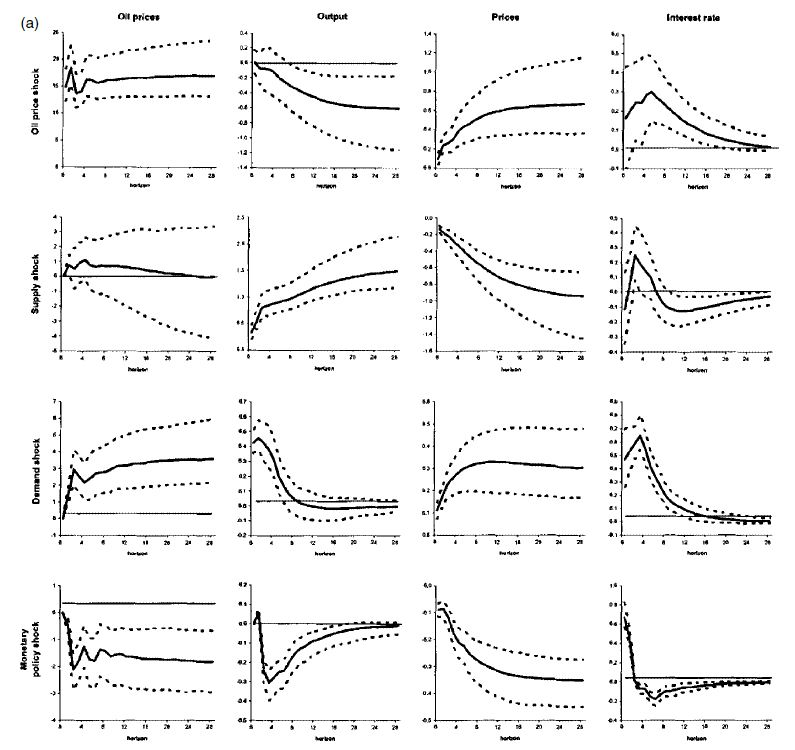
\includegraphics{Capture.jpg}
\caption{Peersman orignial results}
\end{figure}

\bibliography{Tex/ref}





\end{document}
